% DEFT WARS — Game Program Instructions
% Period-style A5 booklet, modeled on early 1980s Atari 2600 manuals.
% Compile: pdflatex manual.tex
\documentclass[10pt]{article}

\usepackage[a5paper,margin=12mm,top=16mm,bottom=16mm]{geometry}
\usepackage[T1]{fontenc}
\usepackage{lmodern}
\usepackage{xcolor}
\usepackage{tikz}
\usepackage{multicol}
\usepackage{microtype}

\definecolor{atariOrange}{HTML}{D75F2E}
\definecolor{atariRed}{HTML}{B8331C}
\definecolor{atariCream}{HTML}{F4E3C0}
\definecolor{atariInk}{HTML}{1A1612}

\pagecolor{atariCream}
\color{atariInk}

\setlength{\parindent}{0pt}
\setlength{\parskip}{4pt}
\setlength{\columnsep}{8mm}

\pagestyle{empty}

% --- Helpers --------------------------------------------------------------
\newcommand{\sectionrule}[1]{%
  \par\vspace{6pt}%
  \noindent\colorbox{atariOrange}{\parbox{\dimexpr\linewidth-2\fboxsep\relax}{\strut\textcolor{atariCream}{\textbf{\textsf{\MakeUppercase{#1}}}}\hfill}}%
  \par\vspace{4pt}%
}

\newcommand{\subhead}[1]{%
  \par\vspace{4pt}%
  \noindent\textbf{\textsf{\MakeUppercase{#1}}}\par\vspace{2pt}%
}

\newcommand{\smallcaption}[1]{{\footnotesize\textsf{#1}}}

% --- Cover-art TikZ panel -------------------------------------------------
\newcommand{\coverpanel}{%
\begin{center}
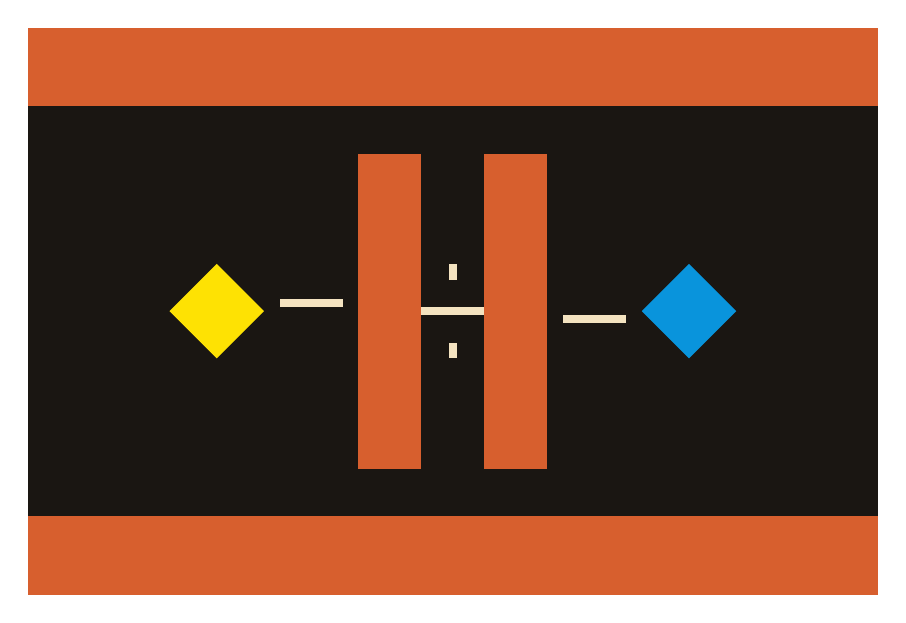
\begin{tikzpicture}
  \fill[atariInk] (-5.4,-3.6) rectangle (5.4,3.6);
  \fill[atariOrange] (-5.4,2.6) rectangle (5.4,3.6);
  \fill[atariOrange] (-5.4,-3.6) rectangle (5.4,-2.6);
  % Two centred wall bars
  \fill[atariOrange] (-1.2,-2.0) rectangle (-0.4,2.0);
  \fill[atariOrange] ( 0.4,-2.0) rectangle ( 1.2,2.0);
  % Yellow diamond (P0)
  \fill[yellow!85!orange] (-3.6,0)
    -- (-3.0,0.6) -- (-2.4,0) -- (-3.0,-0.6) -- cycle;
  % Cyan diamond (P1)
  \fill[cyan!80!blue]   ( 3.6,0)
    -- ( 3.0,0.6) -- ( 2.4,0) -- ( 3.0,-0.6) -- cycle;
  % Missile streaks
  \fill[atariCream] (-2.2,0.05) rectangle (-1.4,0.15);
  \fill[atariCream] ( 1.4,-0.15) rectangle ( 2.2,-0.05);
  % Pickup ball pulsing in the centre
  \fill[atariCream] (-0.05,0.4) rectangle (0.05,0.6);
  \fill[atariCream] (-0.05,-0.6) rectangle (0.05,-0.4);
  \fill[atariCream] (-0.4,-0.05) rectangle (0.4,0.05);
\end{tikzpicture}
\end{center}}

% --- Joystick line drawing ------------------------------------------------
\newcommand{\joystickdiagram}{%
\begin{center}
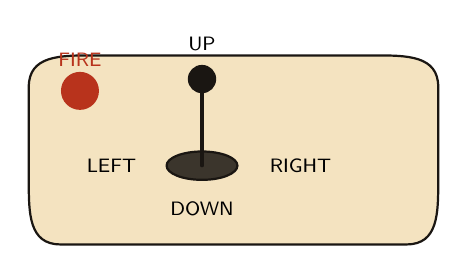
\begin{tikzpicture}[line cap=round, line join=round]
  % Console-shape base
  \draw[atariInk, thick, fill=atariCream]
    (-2.2,-1.0) -- (2.2,-1.0)
    .. controls (2.6,-1.0) and (2.6,-0.6) .. (2.6,-0.2)
    -- (2.6,1.0)
    .. controls (2.6,1.4) and (2.2,1.4) .. (1.8,1.4)
    -- (-1.8,1.4)
    .. controls (-2.2,1.4) and (-2.6,1.4) .. (-2.6,1.0)
    -- (-2.6,-0.2)
    .. controls (-2.6,-0.6) and (-2.6,-1.0) .. (-2.2,-1.0) -- cycle;
  % Stick boot
  \draw[atariInk, thick, fill=atariInk!85!atariCream]
    (-0.4,0.0) ellipse (0.45 and 0.18);
  % Stick
  \draw[atariInk, very thick] (-0.4,0.0) -- (-0.4,1.1);
  \fill[atariInk] (-0.4,1.1) circle (0.18);
  % Fire button (corner red)
  \draw[atariRed, very thick, fill=atariRed]
    (-1.95,0.95) circle (0.22);
  % Direction indicators
  \node[font=\sffamily\scriptsize] at (-0.4,1.55) {UP};
  \node[font=\sffamily\scriptsize] at (-0.4,-0.55) {DOWN};
  \node[font=\sffamily\scriptsize] at (-1.55,0.0) {LEFT};
  \node[font=\sffamily\scriptsize] at ( 0.85,0.0) {RIGHT};
  \node[font=\sffamily\scriptsize, atariRed] at (-1.95,1.35) {FIRE};
\end{tikzpicture}
\end{center}}

% --- Console switch panel -------------------------------------------------
\newcommand{\switchpanel}{%
\begin{center}
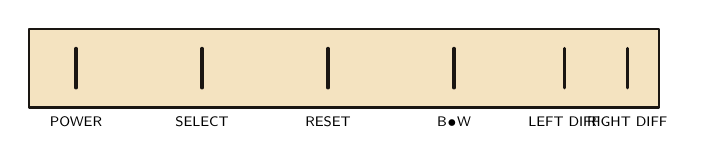
\begin{tikzpicture}[line cap=round, line join=round]
  \draw[atariInk, thick, fill=atariCream] (0,0) rectangle (8.0,1.0);
  \foreach \x/\lbl in {0.6/POWER, 2.2/SELECT, 3.8/RESET, 5.4/B$\bullet$W/COL, 6.8/LEFT DIFF, 7.6/RIGHT DIFF}{%
    \draw[atariInk, very thick] (\x,0.25) -- (\x,0.75);
    \node[font=\sffamily\tiny] at (\x,-0.18) {\lbl};
  }
\end{tikzpicture}
\end{center}}

\begin{document}

% =======================================================================
% PAGE 1 — COVER
% =======================================================================
\begin{center}
\vspace*{2mm}
{\sffamily\bfseries\fontsize{24}{28}\selectfont \textcolor{atariOrange}{DEFT WARS}}\par
\vspace{2mm}
{\sffamily\small TWO-PLAYER COMBAT FOR THE HOME}\par
\vspace{8mm}
\coverpanel\par
\vspace{8mm}
{\sffamily\bfseries GAME PROGRAM INSTRUCTIONS}\par
\vspace{2mm}
{\sffamily\footnotesize MODEL DW-2600 \textbullet{} 4K ROM CARTRIDGE}\par
\vspace{4mm}
{\sffamily\footnotesize FOR USE WITH ATARI 2600 \textregistered{} VIDEO COMPUTER SYSTEM\\AND COMPATIBLE NTSC HARDWARE}
\end{center}

\newpage

% =======================================================================
% PAGE 2 — INSIDE COVER / WELCOME
% =======================================================================
\sectionrule{Welcome to DEFT WARS}

Two pilot diamonds — one yellow, one cyan — duel in the centre of an
asymmetric arena. Centred mirrored walls bend missiles back at their
shooters, and the reckless are punished by collisions that leave them
stunned and slowed. Press the fire button on either joystick at the
title screen and the match begins.

A round ends when a missile lands on its target. The first pilot to land
{\bfseries 8 hits} wins the game.

\subhead{Loading the Game}
\begin{enumerate}\itemsep0pt
\item Make sure the console power is OFF.
\item Insert the DEFT WARS cartridge firmly into the slot.
\item Plug the controllers into the LEFT and RIGHT joystick ports.
\item Switch the power ON. The title screen will read DEFT WARS with
      a large 1 (or 2) below it indicating the game variation in effect.
\item Press SELECT to toggle between Game 1 and Game 2.
\item Press FIRE on a joystick to begin.
\end{enumerate}

\subhead{Title Screen at a Glance}
\begin{itemize}\itemsep0pt
\item {\sffamily\bfseries DEFT WARS} \,---\, the game wordmark, full width.
\item A red {\sffamily 1} or {\sffamily 2} \,---\, the active GAME VARIATION.
\item Tap SELECT to flip between them. Press FIRE to start.
\end{itemize}

\newpage

% =======================================================================
% PAGE 3 — GAME PLAY
% =======================================================================
\sectionrule{Game Play}

\begin{multicols}{2}
\subhead{Movement}
The joystick steers your pilot in any of eight directions with realistic
momentum: holding a direction accelerates you up to a comfortable cruising
speed, and releasing it lets friction bring you to rest. You cannot
leave the visible play field.

\subhead{Firing Missiles}
Pressing FIRE while the joystick is held in any direction launches a
single missile from your pilot in that exact direction. Each pilot may
have only ONE missile in flight at a time. The missile travels for about
half a second before disintegrating, even if it hits nothing.

\subhead{Walls}
Each round draws between one and two centred mirrored walls in randomly
chosen vertical positions, lengths, and colours. Walls block your pilot
\textbf{absolutely}: a hit reverts you a step and zeros your speed. They
also act as missile reflectors --- a missile striking a wall bounces off
at the complementary angle and continues until its half-second life
runs out.

\subhead{Player Collisions}
If two pilots collide, both bounce apart with a satisfying low-pitched
\textit{boing}. The faster of the two has its velocity halved and both
pilots flicker to a hollow `outline' frame for a moment as they recover.
While stunned, neither pilot accepts joystick input.

\subhead{The Pickup Item}
Every five to nine seconds a pulsing item appears somewhere clear of the
walls. The item alternates between a wide block (a `+') and a small
dot (an `x'). Either pilot can grab it by flying through it.

When grabbed, the item randomly either {\bfseries gives} the picker a
free point (with a high-pitched chime) or {\bfseries takes one away}
(with a low-pitched bonk). Scores cannot fall below zero. Whoever grabs
it first wins the toss.

\subhead{Winning a Round}
A missile that strikes the opposing pilot scores 1 point for the
attacker. The screen pauses briefly before both pilots are repositioned
randomly on their own side of the play field for the next round.

\subhead{Winning the Game}
The first pilot to reach {\bfseries 8 points} wins the match. The
winning pilot then erupts into a four-second rainbow celebration,
auto-firing missiles in random directions, before the screen returns to
the title for a new game.
\end{multicols}

\newpage

% =======================================================================
% PAGE 4 — USING THE CONTROLLERS
% =======================================================================
\sectionrule{Using the Controllers}

Use a standard ATARI {CX-40} joystick or compatible. Hold the stick so
the red {\bfseries FIRE} button is in the upper-left corner.

\joystickdiagram

\subhead{The Console Switches}
\switchpanel
\begin{itemize}\itemsep0pt
\item {\bfseries POWER} --- OFF before inserting or removing the cartridge.
\item {\bfseries SELECT} --- {Title screen only.} Toggles between Game 1
      and Game 2. The variation digit on the title screen updates immediately.
\item {\bfseries GAME RESET} --- {Title screen only, alongside FIRE.}
      Starts a fresh match.
\item {\bfseries TV TYPE (B$\bullet$W / COLOR)} --- Cosmetic only on
      this title.
\item {\bfseries LEFT \& RIGHT DIFFICULTY} --- Selects per-pilot
      acceleration. {\sffamily A (PRO)} accelerates every frame.
      {\sffamily B (NOVICE)} accelerates every other frame, making the
      pilot slower to start moving and slower to reverse direction.
\end{itemize}

\newpage

% =======================================================================
% PAGE 5 — GAME VARIATIONS
% =======================================================================
\sectionrule{Game Variations}

\begin{center}
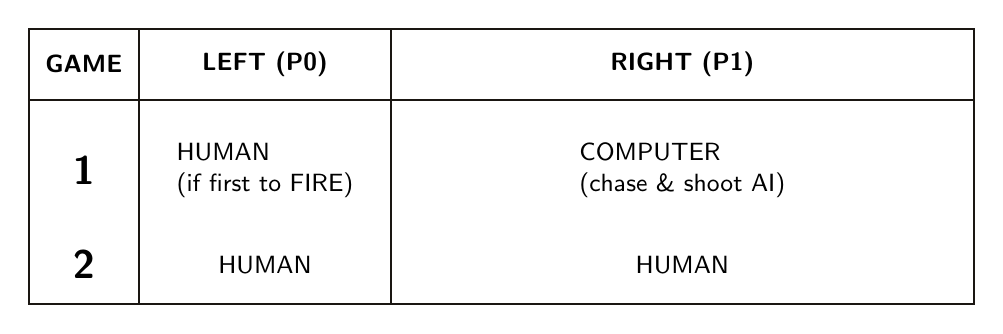
\begin{tikzpicture}
  \draw[atariInk, thick] (0,0) rectangle (12.0,3.5);
  \draw[atariInk, thick] (0,2.6) -- (12.0,2.6);
  \draw[atariInk, thick] (1.4,0) -- (1.4,3.5);
  \draw[atariInk, thick] (4.6,0) -- (4.6,3.5);

  \node[font=\sffamily\bfseries\small] at (0.7,3.05) {GAME};
  \node[font=\sffamily\bfseries\small] at (3.0,3.05) {LEFT (P0)};
  \node[font=\sffamily\bfseries\small] at (8.3,3.05) {RIGHT (P1)};

  \node[font=\sffamily\Large\bfseries] at (0.7,1.7) {1};
  \node[font=\sffamily\small,align=left] at (3.0,1.7) {HUMAN\\(if first to FIRE)};
  \node[font=\sffamily\small,align=left] at (8.3,1.7) {COMPUTER\\(chase \& shoot AI)};

  \node[font=\sffamily\Large\bfseries] at (0.7,0.5) {2};
  \node[font=\sffamily\small] at (3.0,0.5) {HUMAN};
  \node[font=\sffamily\small] at (8.3,0.5) {HUMAN};
\end{tikzpicture}
\end{center}

\subhead{Game 1 --- Single Player vs.\ Computer}
Whichever joystick presses FIRE first becomes the human pilot; the other
joystick's pilot is taken over by the computer. The computer chases the
human's position with a small dead-zone and fires periodically when its
missile slot is free. Use the LEFT or RIGHT DIFFICULTY switch on your
own side to throttle your acceleration if you find the controls
oversensitive.

\subhead{Game 2 --- Two Players}
Both pilots are human. Plug a joystick into each controller port. Press
FIRE on either to start.

\sectionrule{Scoring}
\begin{itemize}\itemsep0pt
\item Successful missile hit on the opposing pilot: {\bfseries +1}.
\item Pickup item, free-point variant: {\bfseries +1}, high chime.
\item Pickup item, penalty variant: {\bfseries -1}, low bonk
      (clamped at zero).
\item First pilot to {\bfseries 8} points wins. The score band at the
      top of the screen shows both pilots' running totals at all times.
\end{itemize}

\newpage

% =======================================================================
% PAGE 6 — HELPFUL HINTS
% =======================================================================
\sectionrule{Helpful Hints}

\begin{multicols}{2}
\subhead{1. Use the Walls}
A missile that strikes a wall reflects off at the complementary angle.
A skilled pilot will line up shots that bounce around the opposing
pilot's cover.

\subhead{2. Keep Moving}
A stationary pilot is an easy target. Use the natural friction in the
movement model to drift through tight spaces and unpredictable arcs.

\subhead{3. Watch the Pickup Pitch}
The pickup chime tells you whether a grabbed item helped you or hurt
you: \textit{high} = +1, \textit{low} = -1. If your opponent is leading,
let \textbf{them} grab it first --- it might cost them a point.

\subhead{4. Don't Crowd the Walls}
Wall transitions and PF patterns vary every round. A wall that looks
like a thin bar one round may be a thick block the next. Reposition
when the layout changes.

\subhead{5. Difficulty Is Per-Pilot}
You can give a younger or less experienced pilot the {\sffamily NOVICE}
side while the more experienced pilot stays on {\sffamily PRO}. Each
side's switch is independent.

\subhead{6. Bouncing Off the Other Pilot}
Slamming into your opponent costs you nothing in points but drains your
speed. Use it deliberately to nudge an opponent toward an incoming
missile.

\subhead{7. Wait Out the Celebration}
At game over, the screen ignores input for four seconds while the
winner celebrates. There is no way to skip it --- enjoy the rainbow.
\end{multicols}

\newpage

% =======================================================================
% PAGE 7 — BACK COVER / SPECIFICATIONS
% =======================================================================
\sectionrule{Specifications}

\begin{center}\sffamily\small
4 KILOBYTE ROM CARTRIDGE \textbullet{} NTSC TIMING\\
SINGLE-BANK, NO BANK-SWITCHING\\
1 OR 2 PLAYERS \textbullet{} 1 OR 2 STANDARD JOYSTICKS\\
USES SELECT, RESET, AND BOTH DIFFICULTY SWITCHES
\end{center}

\sectionrule{Care of Your Cartridge}
\begin{itemize}\itemsep0pt
\item Always switch the console power OFF before inserting or removing
      the cartridge. Inserting under power may damage either device.
\item Do not expose the cartridge to direct sunlight or temperatures
      above 110\,\textdegree{}F.
\item Should the screen show a frozen or scrambled image, switch the
      power off, wait ten seconds, reseat the cartridge and switch
      back on.
\end{itemize}

\sectionrule{Acknowledgements}

DEFT WARS was hand-assembled in 6502 from a standing start over several
focused sessions, with the AI Development Framework providing planning
and review support. The cartridge fits comfortably into 4K with bytes to
spare.

\vspace{4mm}
\begin{center}\sffamily\footnotesize
ATARI\textregistered{} AND THE FUJI LOGO ARE REGISTERED TRADEMARKS\\
OF ATARI INTERACTIVE.\\[2pt]
DEFT WARS IS NOT AFFILIATED WITH OR ENDORSED BY ATARI.\\[6pt]
\textcopyright{} 2026 \textbullet{} HOMEBREW EDITION
\end{center}

\vfill
\begin{center}

\begin{tikzpicture}
  \fill[atariOrange] (0,0) rectangle (4.6,0.5);
  \node[font=\sffamily\bfseries, atariCream] at (2.3,0.25) {GAME OVER --- INSERT QUARTER};
\end{tikzpicture}
\end{center}

\end{document}
